%----------------------------------------------------------
\def\notedate{2023.01.22}
\def\currentauthor{Тришин И.В. (РК6-11М)}
%----------------------------------------------------------
\notestatement{rndhpcpar}{Анализ предыдущих реализаций алгоритма обхода}
%----------------------------------------------------------
\subsubsection{Алгоритм обхода графовой модели в pycomsdk}
Фреймворк pycomsdk предоставляет пользователю программный интерфейс для создания и интерпретации графовых моделей сложных вычислительных методов, созданных по методологии \glsxtrshort{gbse}, на языке python. В нём в процессе обхода графовой модели задействуются следующие сущности:
\begin{enumerate}[label=\arabic*)]
	\item узел графовой модели, соответствующий состоянию данных СВМ (State);
	\item ребро графовой модели, соответствующее функции перехода между состояниями (Transfer);
	\item объект, связывающий ключи в ассоциативном массиве данных (keys_mapping);
	\item объект, отвечающий за стратегию выполнения функций перехода (parallelization_policy).
\end{enumerate}
Функции перехода в \glsxtrshort{gbse} описываются парой $t = <f, p>$, где $f$ -- функция-обработчик, $p$ -- функция-предикат.
В pycomsdk для каждого узла графовой модели $S_i$ хранится список исходящих из него рёбер $T(S_i)$, опционально ссылка на функцию-селектор\cite{SokolovPershin2018} $h_i$ и ссылка на подграф $G_i$. Для каждого ребра $e_{ij}$ хранится вершина, в которую оно входит $S_j$. Кроме того, для каждого узла сохраняется предыдущая история обхода $H_i$, количество необходимых вхождений в неё $N_i^r$, количество совершённых вхождений $N_i^c$ и количество циклов, содержащих данную вершину $L(S_i)$.

В общем виде, без учёта процесса распределения функций перехода между вычислительными ресурсами, процесс обхода графовой модели можно разделить на два этапа:
\begin{enumerate}[label=\arabic*)]
	\item инициализация графовой модели;
	\item выполнение функций перехода.
\end{enumerate}

Алгоритм первого этапа представлен в листинге~\ref{lst:pycomsdk_init}.

\begin{algorithm}[H]
	\caption{Алгоритм инициализации графовой модели}
	\label{lst:pycomsdk_init}
	\begin{algorithmic}[1]
		\Function{IdleRun}{$S_i$, $H$} \Comment{$H$ --текущая накопленная история обхода}
		\If{$G_i \neq \emptyset$}
		\State IdleRun($S_0^{G_i}$, $H$) \Comment{Запуск обхода из начальной вершины подграфа $G_i$}
		\EndIf{}

		\State $N_i^r := N_i^r + 1$
		\If{$N_i^r \neq 1$}
		\If{$H_i \subset H$} \Comment{Проверка на нахождение в цикле}
		\State $L(S_i) := L(S_i) + 1$
		\EndIf{}
		\State \textbf{End}
		\EndIf{}

		\If{$H_i = \emptyset$}
		\State $H_i := H$
		\EndIf{}

		\If{$|T(S_i)| = 1$}
		\State $S_j: e_{ij}\in T(S_i)$
		\State IdleRun($S_j$, $H$)
		\Else{}
		\For{\textbf{each} $e_{ij} \in T(S_i)$}
		\State $S_j: e_{ij}\in T(S_i)$
		\State $H_j := H \cup \left\{S_j\right\}$
		\State IdleRun($S_j$, $H_j$)
		\EndFor
		\EndIf{}

		\EndFunction
	\end{algorithmic}
\end{algorithm}
Можно заметить, что представленный алгоритм представляет собой модифицированный поиск в глубину.

Алгоритм основного обхода графовой модели с данными $D$ представлен в листинге~\ref{lst:pycomsdk_main}.
\begin{algorithm}[H]
	\caption{Основной алгоритм обхода}
	\label{lst:pycomsdk_main}
	\begin{algorithmic}[1]
		\Function{Run}{$D$} \Comment{$S$ -- начальное состояние, $D$ -- данные}
		\State $S = S_0$
		\While{$S \neq \emptyset$} \Comment{Пока не достигнуто конечное состояние}
		\State $F = $ RunState($S$, $D$) \Comment{Получить функцию(-ции) перехода для текущего состояния}
		\State $S = F(D)$ \Comment{Выполнить функции перехода и получить новое состояние}
		\EndWhile
		\EndFunction

		\Function{RunState}{$S_i$, $D$}
		\If{$G_i \neq \emptyset$}
		\State RunState($S_0^{G_i}, D$)
		\EndIf

		\State $N_i^c := N_i^c + 1$
		\If{$N_i^c \neq N_i^r$} \Comment{Если не все необходимые переходы ещё совершены}
		\State \textbf{return} $\empty$
		\EndIf

		\If{$|T(S_i)| = 0$} \Comment{Если из текущего узла нет исходящих рёбер}
		\State \textbf{return} $\empty$
		\EndIf

		\State $U = h_i(D)$ \Comment{Получить набор флагов, разрешающих или запрещающих переходы по исходящим рёбрам}
		\State $T = \emptyset$ \Comment{Инициализировать набор ф-ций перехода, запланированных к выполнению}
		\For{\textbf{each} $u_j \in U$}
		\If{$u_j = true$ \textbf{and} $p_j(D) = true$} \Comment{Если переход разрешён селектором и проверка предикатом прошла успешно}
		\State $T := T \cup \left\{t_j\right\}, t_j \in T(S_i)$
		\EndIf
		\EndFor

		\State $F = $ makeTransfer(parallelization_policy, $T$) \Comment{Получить функции перехода согласно стратегии их выполнения}
		\State \textbf{return} $F$
		\EndFunction
	\end{algorithmic}
\end{algorithm}
Необходимо отметить, что алгоритм упомянутой функции makeTransfer зависит от стратегии выполнения рёбер, поэтому не может быть приведён в общем виде.

В приведённом алгоритме можно выделить следующие особенности.
\begin{enumerate}
	\item Для проверки принадлежности вершины к циклу в ориентированном графе используется история предыдущих посещений, что требует хранения этой истории для каждой из вершин.
	\item Используются рекурсивные вызовы функции обхода, что может затруднить отладку алгоритма.
	\item Решение о том, какие переходы совершать далее, принимается непосредственно при входе в вершину.
	\item Функция перехода планируется к выполнению только при истинности соответствующего предиката. Это позволяет избежать лишних проверок и повышает производительность.
\end{enumerate}

\subsubsection{Алгоритм обхода в новой версии comsdk}
Фреймворк comsdk является ещё одной, исторически более ранней, реализацией программных средств, позволяющих пользователю создавать и автоматически интерпретировать графовые модели сложных вычислительных методов. Данный фреймворк реализован на языке С++. В рамках ВКР бакалавра над данным фрейморком велась работа по обновлению некоторых его компонентов, среди которых так же находится интерпретатор графовых моделей. В рамках ВКР для интерпретатора был разработан обновлённый алгоритм, поддерживающий возможность задействовать различные вычислительные ресурсы для выполнения функций перехода.

В текущей реализации comsdk графовая модель представляется набором узлов -- состояний данных $S_i$, -- рёбер -- функций перехода $t_j$ -- и матрицей смежности $Adj$. С каждым узлом $S_i$ связывается только стратегия выполнения исходящих из него ветвей графовой модели и опционально селектор $h_i$. Для данного алгоритма были разработаны две абстрактные управляющие структуры -- контейнер выполнения и ветвь выполнения. Назначение первой -- отслеживание выполнения ветвей и управление задействованными вычислительными ресурсами. Задача второй -- последовательный обход одной ветви графовой модели, в которой гаратировано отсутствие ветвления. Алгоритмы обхода одной ветви и работы контейнера выполнения представлены на рисунках~\ref{fig:comsdk_branch} и \ref{fig:comsdk_container}.

\begin{figure}[H]
	\centering
	\includegraphics[width=0.9\textwidth]{ResearchNotes/rndhpc_not_par_2022_01_22/flowchart.executionBranch.png}
	\caption{Блок-схема алгоритма обхода одной ветви графовой модели}
	\label{fig:comsdk_branch}
\end{figure}

\begin{figure}[H]
	\centering
	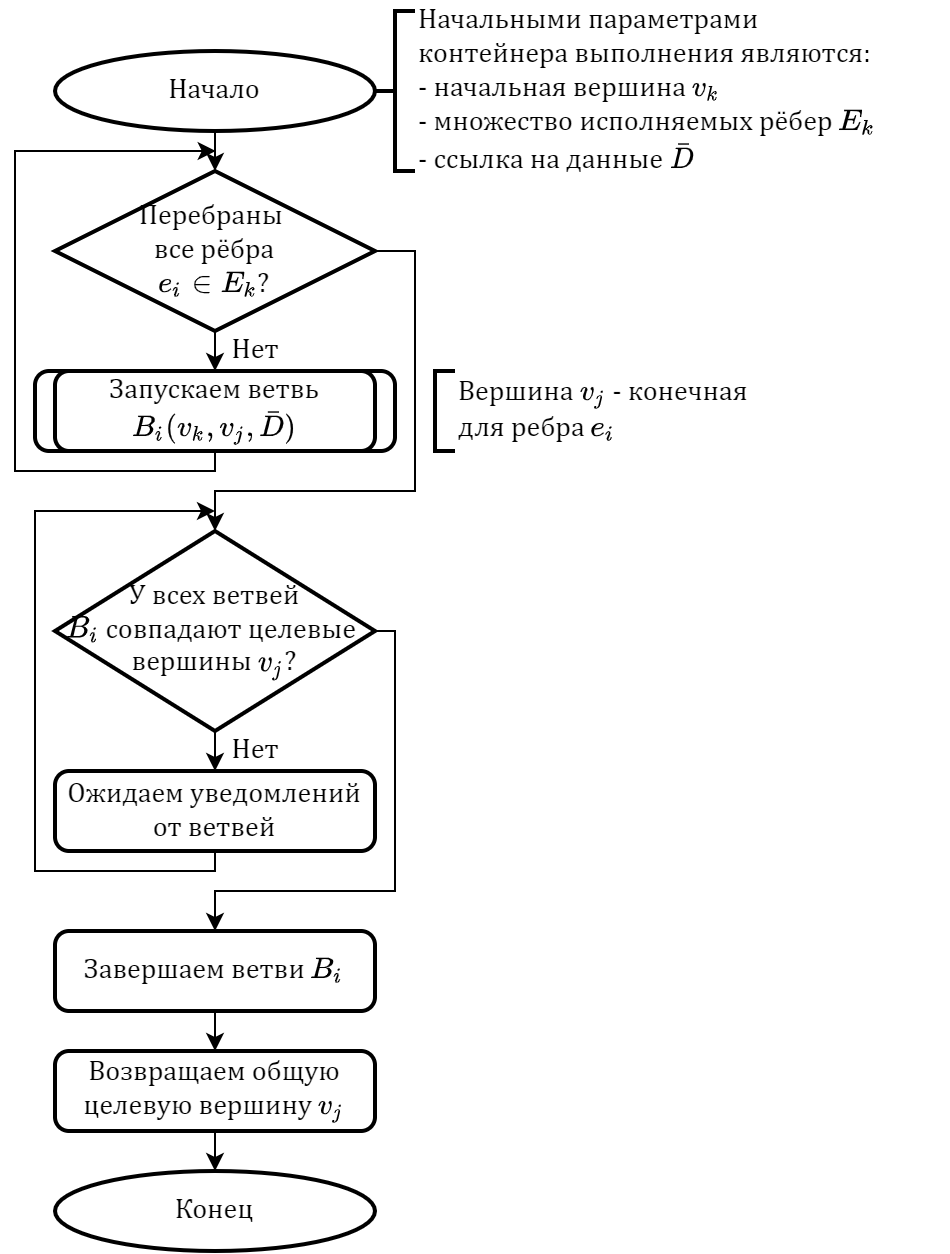
\includegraphics[height=0.6\textheight]{ResearchNotes/rndhpc_not_par_2022_01_22/flowchart.executionContainer.png}
	\caption{Блок-схема алгоритма работы контейнера выполнения для обхода нескольких ветвей графовой модели}
	\label{fig:comsdk_container}
\end{figure}

У разработанного алгоритма можно выделить следующие особенности.
\begin{enumerate}
	\item Структура контейнера даёт разработчику достаточно высокий уровень абстракции при разработке алгоритма обхода. Все особенности взаимодействия с вычислительными ресурсами закладываются в функции запуска ветвей и уведомления контейнера, интерфейс сохраняется общий. Для задействования различных ресурсов достаточно сменить реализацию контейнера.
	\item Контейнеры и ветви создаются рекурсивно, что может создать сложности при отладке.
	\item Алгоритм не устойчив к наличию в графовой модели циклов и в худшем случае может уйти в бесконечную рекурсию.
\end{enumerate}
%----------------------------------------------------------
% Атрибуты задачи
\noteattributes{}
%----------------------------------------------------------